\sub {

Let's consider the proper bracket $\bracksig{[16; 0; 0; 0; 0]}$, which was used in the 2022 NCAA Women's Basketball Tournament Wichita Region, and is shown here: (Sometimes brackets are drawn in the manner below, with teams starting on both sides and the winner of each side playing in the championship game.)

\fig{0.8}{2021 NCAA Basketball Tournament South Region.png}{2022 NCAA Women's Basketball Tournament Wichita Region}{}

The definition of a proper seeding ensures that as long as the bracket goes to chalk (that is, higher seeds always beat lower seeds), it will always be better to be a higher seed than a lower seed. But what if it doesn't go to chalk?

One counter-intuitive fact about the NCAA Basketball Tournament is that it is probably better to be a 10-seed than a 9-seed. (This doesn't violate the proper seeding property because 9-seeds have an easier first-round matchup than 10-seeds, and for further rounds, proper seedings only care about what happens if the bracket goes to chalk, which would eliminate both the 9-seed and 10-seed in the first round.) Why? Let's look at whom each seed-line matchups against in the first two rounds:

\begin{figg}{NCAA Basketball Tournament 9- and 10-seed Schedules}{}
    \centering
    \begin{tabular}{ c | c c }
         Seed & First Round & Second Round \\
         \hline
         9 & 8 & 1\\
        10 & 7 & 2
    \end{tabular}
\end{figg}

The 9-seed has an easier first-round matchup, while the 10-seed has an easier second-round matchup. However, this isn't quite symmetrical. Because the teams are (most likely) drawn from a roughly normal distribution, the difference in skill between the 1- and 2-seeds is far greater than the difference between the 7- and 8-seeds, implying that the 10-seed does in fact have an easier route than the 9-seed.

Nate Silver investigated this matter in full, finding that in the NCAA Basketball Tournament, seed-lines 10 through 15 give teams better odds of winning the region than seed-lines 8 and 9. Of course this does not mean that the 11-seed (say) has a better chance of winning a given region than the 8-seed does, as the 8-seed is a much better team than the 11-seed. But it does mean that the 8-seed would love to swap places with the 11-seed, and that doing so would increase their odds to win the region.

This is not a great state of affairs: the whole point of seeding is confer an advantage to higher-seeded teams, and the proper bracket $\bracksig{[16; 0; 0; 0; 0]}$ is failing to do that. Not to mention that giving lower-seeded teams an easier route than higher-seeded ones can incentivize teams to lose during the regular season in order to try to get a lower but more advantageous seed.

To fix this, we need a stronger notion of what makes a bracket effective than properness. The issue with proper seedings is the false assumption that higher-seeded teams will always beat lower-seeded teams. A more nuanced assumption might look like this:

%does seeding maen the ordering of the teams or placement of the teams in the bracket

\begin{definition}{$t_i$}{}
    For ease of use, in mathematical formulae we sometimes use the notation $t_i$ to refer to the $i$-seed in a tournament.
\end{definition}

\begin{definition}{Strongly Stochastically Transitive}{}
    A seeded list of teams is \textit{strongly stochastically transitive} if for each $i, j, k, \ell$ such that $i \leq j$ and $k \leq \ell$, $$\P(t_i \textrm{ beats } t_\ell) \geq \P(t_j \textrm{ beats } t_k).$$
\end{definition}

A list of teams being strongly stochastically transitive (or SST) captures the intuition that higher-seeded teams ought to be better than lower-seeded teams, and that higher seeds ought to do better against lower seeds than lower seeds do against higher seeds. 

% A quick implication of this is

% \begin{corollary}{}{}
%     If a list of teams is SST, then for each $i < j$, $\P(t_i \textrm{ beats } t_j) \geq 0.5.$
% \end{corollary}

Note that not every set of teams can be seeded to be SST. Consider, for example, the game of rock-paper-scissors. Rock beats paper which beats scissors which beats rock, so no ordering of these ``teams'' will be SST. For our purposes, however, SST will work well enough.

Our new, nuanced alternative a proper bracket is an \textit{ordered bracket}.

\begin{definition}{Ordered Bracket}{}
    A bracket and seeding are \textit{ordered} if, for any SST list of teams, if $i < j$, then $\P(t_i\textrm{ wins the tournament} )\geq \P(t_j\textrm{ wins the tournament}).$
\end{definition}

In many ways, a bracket being ordered is the strongest thing we can want without making any ``moral'' judgements. It might be unclear (and vary by situation) whether a it is better for a format to almost always declare the most-skilled team the winner, or to give each team roughly the same chance of winning, or anywhere in between. But certainly, better teams should win more, which is what the ordered bracket stipulation requires.

In particular, a bracket being ordered is a stronger claim than it being proper.
%/A vs /B
\theo{}{Every ordered bracket is proper.}{
    %this proof is el garbo pants
    Let $\A$ be an ordered $n$-team bracket with $r$ rounds.\\
    
    Consider a list of teams such that every team wins every game with probability 0.5. These teams are SST. A team that plays their first game in the $i$th round will win the tournament with probability $(\frac{1}{2})^{r-i}$, so teams that get more byes will have a higher probability to win the tournament than teams with fewer byes. Thus, higher-seeded teams must have more byes than lower-seeded teams, so in each round, the teams with byes must be the highest-seeded teams that are still alive. Thus, condition (1) is met.\\



    %i vs j
    %k vs l
    %i < k, j < l
    %i < j
    %


    % i < j < k < l s.t. 

   % Now assume for contradiction that condition (2) is not met for the first time in round $s$, so there exists seeds $i < j < k < \ell$ such that in round $s$, if the bracket goes to chalk, they are each paired up against each other, but in some configuration other than $t_i$ vs $t_\ell$ and $t_j$ against $t_k$. Now consider the following SST matchup table: games between teams 
    %
    %$t_i$ played $t_j$ and $t_k$ played $t_\ell,$ where $i < k$ but $j < \ell.$ Without loss of geneeralization, assume $i < j.$  

    Consider an arbitrary round $i$. Let $t_1, ... t_m$ be the teams that would be playing in this round if the bracket went to chalk so far, ordered by seed. Consider the following SST matchup table on the teams remaining: every team wins every game with probability 0.5, except for games involving $t_m$, who is guarenteed to lose every game they play. Then, each team playing this round will win the tournament with probability $(\frac{1}{2})^{r-i},$ other than $t_m$ who wins with probability $0$ and the team playing $t_m$ who wins with probability $(\frac{1}{2})^{r-i-1}.$ Since that team has a better chance of winning than the other teams playing this round, and $\B$ is ordered, the team playing $t_m$ has to be the highest-seeded team playing this round, which is $t_1.$  We can then build more SSTs, adding the next-lowest seed as also losing every game they play to ensure that they must play the next-highest seed, until we've shown that all the teams playing this round must be matched up according to condition (2).\\

    Thus $\B$ satisfies both conditions, and so is a proper bracket.
}{ordered_proper}

With Theorem \ref{th:ordered_proper}, we can use the language of bracket signatures to describe ordered bracket without concerns over collision. Now we attempt to fully characterize the space of ordered brackets, beginning by constructing and proving the orderedness of three particularly important brackets.

We begin with the unique one-team bracket.

\fig{1}{one_team.png}{The One-Team Bracket $\bracksig{[1]}$.}{}
\theo{}{The one-team bracket $\bracksig{[1]}$ is ordered.}{Since there is only team, the ordered bracket condition is vacuously true.}{}

Next we look at the unique two-team bracket.

\fig{1}{two_team.png}{The Two-Team Bracket $\bracksig{[2; 0]}$.}{}
\theo{}{The two-team bracket $\bracksig{[2; 0]}$ is ordered.}{Let $\A = \bracksig{[2; 0]}.$ Then,
\begin{align*}
   \P[t_1 \textrm{ wins } \A] = \P[t_1 \textrm{ beats } t_2] \geq 0.5 \geq \P[t_2 \textrm{ beats } t_1] = \P[t_2 \textrm{ wins } \A],
\end{align*}    
so $\A$ is ordered.
}{}

And thirdly, we show that the balanced four-team bracket is ordered.

\fig{1}{four_team.png}{The Four-Team Bracket $\bracksig{[4; 0; 0]}$.}{}
\theo{}{The four-team bracket $\bracksig{[4; 0; 0]}$ is ordered.}{Let $\A = \bracksig{[2; 0]}.$ Let $p_{ij}$ be the probability that the $i$-seed beats the $j$-seed. Then,
\begin{align*}
    \P[t_1 \textrm{ wins } \A] &= p_{14} \cdot (p_{23}p_{12} + p_{32} p_{13})\\
    &= p_{14}p_{23}p_{12} + p_{14}p_{32} p_{13}\\
    &\geq p_{14}p_{23}p_{21} + p_{24}p_{41} p_{23}\\
    &= p_{23} \cdot (p_{14}p_{21} + p_{41}p_{24})\\
    &= \P[t_2 \textrm{ wins } \A]
\end{align*}
\begin{align*}
    \P[t_2 \textrm{ wins } \A] &= p_{23} \cdot (p_{14}p_{21} + p_{41} p_{24})\\
    &\geq p_{32} \cdot (p_{14}p_{31} + p_{41} p_{34})\\
    &= \P[t_3 \textrm{ wins } \A]
\end{align*}
\begin{align*}
    \P[t_3 \textrm{ wins } \A] &= p_{32} \cdot (p_{14}p_{31} + p_{41} p_{34})\\
    &= p_{32}p_{14}p_{31} + p_{32}p_{41} p_{34}\\
    &\geq p_{42}p_{23}p_{41} + p_{32}p_{41} p_{43}\\
    &= p_{41} \cdot (p_{23}p_{42} + p_{32}p_{43})\\
    &= \P[t_4 \textrm{ wins } \A]
\end{align*}

Thus the four-team bracket $\bracksig{[4; 0; 0]}$ is ordered.
}{}

%excerize, try [8;0;0;0]. Dont try too hard though!$

Now we stop describing particular ordered brackets in favor of a more general result. The idea of the upcoming theorem is to combine two smaller ordered brackets together into one larger ordered bracket by having the winner of one of the brackets slot into the lowest seed starting line of the other. This is depicted in Figure \ref{fig:ordered_bracket_staple}.

\fig{.95}{ordere_bracket_sum.png}{The Setup of Theorem \ref{th:order_bracket_sum}}{ordered_bracket_staple}

\theo{}{If $\A$ and $\B$ are $n$- and $m$-team ordered brackets, respectively, we can construct an $(n + m - 1)$-team oredered bracket by replacing the lowest seed in $\B$ with the entire bracket $\A$ (lowering the seed of each team in $\A$ by $m-1$).}{
Let $\C$ be the bracket formed by merging $\A$ and $\B.$ We divide proving that $\C$ is ordered into proving three substatements:
\begin{enumerate}
    \item For $i < j < m,$ $\P(t_i \textrm{ wins }\C) \geq \P(t_j \textrm{ wins }\C)$
    \item $\P(t_{m-1} \textrm{ wins } \C) \geq \P(t_m \textrm{ wins } \C)$
    \item For $m \leq i < j,$ $\P(t_i \textrm{ wins } \C) \geq \P(t_j \textrm{ wins } \C)$
\end{enumerate}
Together, these show that $\C$ is ordered.\\

We begin with the first substatement. Let $i < j < m.$ Then,
\begin{align*}
    \P(t_i \textrm{ wins }\C) &= \P(t_i \textrm{ wins }\B)\\
    &= \sum_{k=n}^{n+m-1} \P(t_i \textrm{ wins }\B \;\mid\; t_k \textrm{ wins } \A)\cdot \P(t_k \textrm{ wins } \A)\\
    &\geq \sum_{k=n}^{n+m-1} \P(t_j \textrm{ wins }\B \;\mid\; t_k \textrm{ wins } \A)\cdot \P(t_k \textrm{ wins } \A)\\
    &=\P(t_j \textrm{ wins }\B)\\
    &=\P(t_j \textrm{ wins }\C)
\end{align*}
The first and last equalities follow from the structure of $\C,$ and the inequality follows from $\B$ being ordered.\\

Now the second substatement.
\begin{align*}
    \P(t_{m-1} \textrm{ wins }\C) &= \P(t_{m-1} \textrm{ wins }\B)\\
    &\geq \P(t_{m} \textrm{ wins }\B \;\mid\; t_{m} \textrm{ wins }\A)\\
    &\geq \P(t_{m} \textrm{ wins }\B \;\mid\; t_{m} \textrm{ wins }\A) \cdot \P(t_{m} \textrm{ wins }\A)\\
    &= \P(t_{m} \textrm{ wins }\C)
\end{align*}
The equalities follow from the structure of $\C,$ and the first inequality follows from $\B$ being ordered.\\

Finally we show the third substatement. Let $m \leq i < j.$ Then,
\begin{align*}
    \P(t_i \textrm{ wins }\C) &= \P(t_i \textrm{ wins }\B \;\mid\; t_i \textrm{ wins } \A)\cdot \P(t_i \textrm{ wins } \A)\\
    &\geq \P(t_i \textrm{ wins }\B \;\mid\; t_i \textrm{ wins } \A)\cdot \P(t_j \textrm{ wins } \A)\\
    &\geq \P(t_j \textrm{ wins }\B \;\mid\; t_j \textrm{ wins } \A)\cdot \P(t_j \textrm{ wins } \A)\\
    &= \P(t_j \textrm{ wins }\C)
\end{align*}
The equalities follow from the structure of $\C$, the first inequality from $\A$ being ordered, and the second inequality from the teams being SST.\\

We have shown all three substatements, and so $\C$ is ordered.
}{order_bracket_sum}

\begin{corollary}{}{}
    If $\A = [a_0; ...; a_r]$ and $\B = [b_0; ...; b_s]$ are ordered brackets, then $\C = [a_0; ...; a_r + b_0 - 1; ...; b_s]$ is an ordered bracket as well.
\end{corollary}

We can then construct the set of brackets that we have thus far shown are ordered. We do this by starting with $\{\bracksig{[1]}, \bracksig{[2; 0]}, \bracksig{[4; 0; 0]}\}$ and then repeatedly applying the above theorem on the set to expand it. In other words,

\begin{corollary}{}{construct_order}
    Any bracket signature formed by the following process is ordered:
    \begin{enumerate}
        \item Start with the list $\bracksig{[0]}$ (note that this not yet a bracket signature).
        \item As many times as desired, prepend the list with $\bracksig{[1]}$ or $\bracksig{[3; 0]}.$
        \item Then, add 1 to the first element in the list, turning it into a bracket signature.
    \end{enumerate}
\end{corollary}

Corollary \ref{th:construct_order} uses the tools that we have developed so far to demark a set of brackets as ordered. Somewhat suprisingly, this set is complete: any bracket not reachable using the process in Corollary \ref{th:construct_order} is not ordered.

\lemm{}{
    If $\A$ is an $r$-round ordered bracket and two games are played in round $s$, then the winners of those games must play each other in round $s+1.$ Further, this must the only game of round $s+1$. 
}{
    Let $m$ be the number of teams that are still alive in $\A$ after round $s.$ Because $\A$ is proper, we know that if the bracket goes to chalk, $t_m$ will play $t_{m+1}$ in round $s$.\\

    Now, assume for contradiction that two games are played in round $s$ but the winners of those games do not play each other in the following round. So let $k<\ell$ such that, if the bracket goes to chalk, $t_k$ plays $t_\ell$ in round $s$, but the winner of that game doesn't play the winner of the $t_m$ game in round $s+1.$ In fact, let $k$ be the lowest such seed. Finally, let $i$ and $j$ be such that if the bracket goes to chalk, in round $s + 1$, $t_i$ will play $t_m$ and $t_j$ will play $t_k.$\\

    The situation so far (assuming all omitted games go chalk):
    \begin{center}
        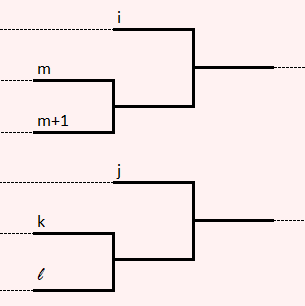
\includegraphics{images/two_must_play_ordered.png}
    \end{center}

    We can use $\A$'s properness to determine that $i < j < k < m < m + 1 < \ell.$\\

    Consider now the following SST set of matchups: games between two teams seeded $\ell + 1$ or higher are coin flips, games between $t_\ell$ and teams seeded between $t_{\ell+1}$ and $t_k$ are coin flips, and all other games are always won by the higher seed.\\

    Let's calculate the probability of $t_i$ and $t_j$ winning the tournament. $t_i$ will auto-win any games the have prior to round $s+1$, and then have to win $r - s$ coin flips in order to win the tournament. This happens with probability $0.5^{r-s}.$\\

    $t_j$ will also win all of its games prior to round $s+1$, also has to win a coin flip for each games in round $s+2$ or later. For round $s+1$, however, half the time $t_j$ will be matched up with $t_k$, which is a coin flip, but half the time they will be matched with $t_k$, which is an auto-win. Thus, $t_j$ will win the tournament with probability $0.75(0.5)^{r-s-1}.$\\

    Therefore, $t_j$ has a better chance of winning the tournament than $t_i$ does, despite $t_i$ being higher seeded, so $\A$ is not ordered, completing the contradiction. Thus if two games are played in round $s$, the winners of those games must play each other in round $s+1.$\\

    This immediately implies that at most two games can be played in each round of an ordered bracket.\\
    
    Finally, we know that this can be the only game played in round $s+1$ because if there was another game, it would have to be between two teams that are higher-seeded than the two teams who won in the previous round, meaning that round violated condition (2).
}{two_must_play}

And now the main theorem,

\theo{}{
    The only ordered brackets are those described by Corollary \ref{th:construct_order}.
}{
    Corollary \ref{th:construct_order} describes all proper brackets in which each round either has only game, or has two games but is immediately followed by a round with only one game. A proper bracket not described by Corollary \ref{th:construct_order} would thus have to include a round with two or more games followed by another round with two or more games, violating Lemma \ref{th:two_must_play}.
}{limit_order}

Theorem \ref{th:limit_order} is both exciting and disapointing. On one hand, it means that Corollary \ref{th:construct_order} fully describes the set of ordered brackets, making it easy to, e.g., check whether a given bracket is ordered or not. On the other hand, because in an ordered bracket at most three teams can be introduced each round, the length of the shortest ordered bracket on $n$ teams grows linearly with $n$ (rather than logarithmically as is the case for proper brackets). This means that if we want a bracket on many teams to be ordered, we risk forcing lower-seeded teams to play large numbers of games, and we only permit the top seeded teams to play a few. For example, if the 2022 NCAA Women's Basketball Wichita Region wanted to use an ordered bracket, rather than just a proper one, the shortest bracket they could use would be $\bracksig{[4; 0; 3; 0; 3; 0; 3; 0; 3; 0; 0]},$ which is played over a whopping ten rounds.

\fig{.475}{ordered_sixteen.png}{The Shortest Sixteen-Team Ordered Bracket}{}

%Because of this, few leagues uses ordered brackets, and those who do usually use them by accident. One such as the 2023 College Football Playoffs which uses a $\bracksig{[4; 0; 0]}$ bracket. (Given that all four-team proper brackets are ordered, it seems unlikely that this was an intentional choice. In fact, starting in 2025, the College Football Playoffs will be moving to the unordered $\bracksig{[8; 4; 0; 0; 0]}$ bracket.) One notable exception to this is the Korean Baseball League, which does ele


%korean baseball fig
}